
\begin{abstract}
	Arbeta om patent ...
\end{abstract}	
	
	
\section{Inledning}

Patent har antagit en central roll i den globala marknaden.
Det ansöks om fler patent än någonsin, och i en så hög takt att patentutfärdarna
får svårt att hinna med \cite{uspto_number}. Se figur \ref{fig:holg} som visar antalet patentansökningar i olika länder där USA och kina ökar markant, märk skillnade in i gradering mellan länderna\footnote{grafen är tagen ifrån \cite{holg}}.
Patent har blivit ett viktigt strategiskt verktyg för företag att skydda sina
intressen, stärka sin förhandlingsposition, generera inkomster genom
licensering, och att hindra konkurrenter från att äntra och utvecklas på
marknaden. 
Den senaste tiden har flera stora patentstrider mellan teknikföretag
uppmärksammats i media, och detta har gett liv åt debatten om vilken nytta
patent tillför samhället.
Att patent har stor betydelse i den globala ekonomin ses tydligt genom att
de utvecklade länderna drev på införandet av starkare patentskydd i
internationella förhandlingar \cite{ove}. 

\begin{figure}[h!]
  
  \centering
    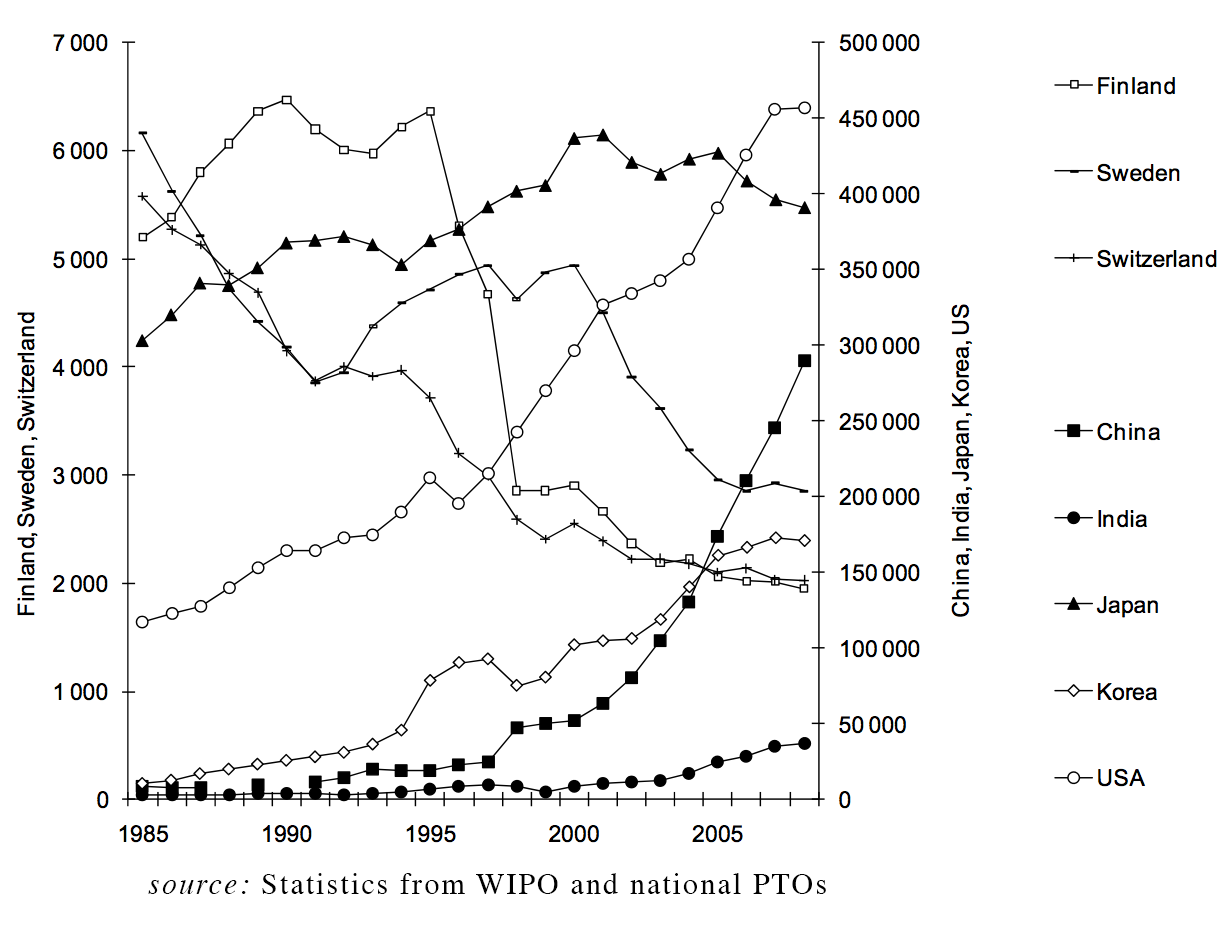
\includegraphics[width=1.15\textwidth]{../holg.png}
	\caption{Patentansökningar per år i olika länder}
	\label{fig:holg}
\end{figure}




\section{Syfte och frågeställningar}

Arbetets syfte är att utreda det historiska ursprunget till patentsystemet och
granska det kritiskt i ljus av den aktuella debatten kring patent.
Vi vill också utreda hurvida maximet att ett patent är ett kontrakt mellan en
uppfinnare och allmänheten där allmänheten tillåter att uppfinnaren har ensam
ekonomisk vinning av uppfinningen i utbyte mot att han delger kunskap till
allmänheten, public domain, har historisk förankring.

Alltså vill vi besvara frågan om patent historiskt uppkommit för att gynna
allmänheten eller av annan anledning. Våra övriga frågeställningar inkluderar:
När började patent att utfärdas? Vilka alternativ fanns innan patent?
Vilka har haft makt över, och vilka har gynnats av patentsystemet?

Första delen i rapporten beskriver
uppkomsten av vad vi idag skulle kalla patent i renässansens Italien.
Andra delen följer utvecklingen av patentsystemet i England under perioden
1500-1800 här rör det sig om ett privilegie beviljat av kungen. Rapportens tredje del går vidare till USA, och beskriver patentsystemets förändring med tiden där. Därefter i avsnitt 5 behnadlar vi nutida handelsvtal och hur dagens patentlandskap ser ut. Dessa delar sammanfattas i korta listor som enkelt kan jämföras. Rapporten avslutat med en reflektion över viktiga likheter och skillnader mellan de olika interationerna och söker besvara våra frågeställningar. 
 %avsnitt inte siffror utan lables så det inte blir dumt i huvut
 
 %tre faser privilegier, kung -> privilegier stat -> nu
I rapporten beskrivs tre distinkta faser av patentsystemet: engelska kungens privilegiesystem på medeltiden, england och usas patentsystem på 1800-talet och slutligen det moderna patentsystemet i USA, Eu och Kina. Dessa tre innefattar helt olika definintioner och synsätt på ett patent och ger en god uppfattning om patentsystemets utveckling från privilegium under engelska kungen till en rigid rättighet idag, och 1800-talets system illustrerar en övergångsfas mellan de två, när rättighetsprincipen först annamats. 

Dessa faser behandlas i kronologisk ordning där det historiska begreppet patent beskrivs i avsnitt \ref{sec:lit} och vidareutvecklas i en redogörelse för patentsystemet på medeltiden i avsnitt \ref{sec:med}. Därefter behandlas privilegiemodellen för patent i medeltidens england i avsnitt \ref{sec:eng} och vi följer där utvecklingen mot 1800-talets första rättighetssystem. Vidare behandlas samma övergång i USA i avsnitt \ref{sec:usa}. Sedan beskriver vi det moderna patentsystemet i avsnitt \ref{sec:mod} och hur det används av företag på den globala marknaden i avsnitt \ref{sec:ip}. Avslutningsvis sammanfattas de olika faserna av patentsystemets uppkomst i avsnitt \ref{sec:samm} och en jämförelse presenteras i avsnitt \ref{sec:disk} där rapporten besvarar frågeställningarna.
 
 %varför de länder vi har, varför inte nadra länder
 %brafen som ahn hade på länderna
 
 Ett patent är en ensamrätt att utnyttja en ny uppfinning. Det innebär att ingen
 annan får utnyttja uppfinningen genom att tillverka, sälja eller importera 
 uppfinningen utan patentinnehavarens tillstånd. Det ses också som uppfinarens naturliga rättighet att skydda sin upptäckt med ett patent. Patent är en av flera sorters
 immaterialrätt, men vi har valt att begränsa vår studie till patent enligt
 definitionen ovan, och behandlar Intelectual Property endast i modern tid då det är väl sammankopplade ämnen. Men vi undviker att beröra närliggande koncept som upphovsrätt.

\section{Metod och källor}
%ssction?
%*står inget om metod, vad har vi för metod?

Våra främsta källor för patentsystemets historia är MacLeod \cite{macleod},
Bracha \cite{bracha} och Nard \cite{nard}.

Christine MacLeod sammanfattar brittiska patentsystemets utveckling mellan 
1600 och 1900 i rapporten \emph{Patents and Industrialisation - An Historical 
Overview of the British Case, 1624-1907}. Vi fann denna på brittiska 
Intellectual Property Offices hemsida och drar slutsatsen att detta är en 
rapport skriven för IPO. MacLeod är professor i historia vid University of 
Bristol i England varför vi finner rapporten trovärdig.

Oren Bracha ger en detaljrik och klarsynt bild av patentsystemets utveckling 
från monarkiska privilegierna i England i sin doktorsavhandling \emph{Owning 
Ides: A History of Angle-American Intellectual Property}. Bracha är nu 
juridikprofessor vid University of Texas School of Law. Avhandlingen citerar 
ofta ett annat av MacLeods verk så dessa två källor tar del av samma 
historieskrivning, vilket inte är så konstigt då få diskrepanser har upptäckts 
mellan olika källor.

Craig Allen Nard har skrivit boken \emph{The law of patents} som främst 
behandar juridiken bakom dagens patentsystem, men också viger ett kapitel åt 
patentsystemets uppkomst. Nard är juridikprofessor vid Case Western Reserve.

Dessa källor anses av oss vara trovärdiga då samtliga författare är erkända 
professorer inom sina fält och texterna i sig uppvisar hög akademisk standard. 
I de fall som dessa huvudkällor refererar vidare till andra verk för 
specifika detaljer har vi sökt att läsa originalkällan men i de fall dessa ej 
varit tillgängliga har vi litat på andrahandskällor.

%*också förklara viktiga termer: case law, first-to-X


%varför england usa eu och inte andra länder?
%var ska detta vara?




\section{Begreppet Patent} %och IPR i historien? -> transaktionskostnad idéer
\label{sec:lit}

Historiskt sett kommer termen patent från latinets \emph{litterae patentes} som
betyder öppet brev. Kopplingen till dagens patent är att medeltida monarker gav
ut 'privilegier', land, titlar, friheter och informerade om detta genom ett
öppet brev, \emph{litterae patentes}, där det kungliga sigillet placerades på
ett sådant sätt att brevet skulle kunna läsas utan att bryta sigillet\cite{blackstone} (ett vanligt brev förseglas av sigillet). Breven var också uttryckligen adresserade till 
vemhelst som läser det, alltså alla. Dessa privilegier kunde innefatta ensamrätt
att sälja en viss vara. Ordet patent har levt kvar genom historien till 
att nu innebära kommersiell ensamrätt till uppfinningar men även andra områden som design och proceser. 

När vi talar om patent i historisk mening är det viktigt att poängtera att det 
snarare är \emph{litterae patentes} med koppling till de tidigare 
privilegierna än patent i modern bemärkelse. Skiftet till det moderna perspektivet skedde löpande under början av 1800-talet och skulle fastslås i lagstifning runt mitten av 1800.
